Pour valider notre modèle, nous avons développé une simulation basée sur un graphe.
Chaque machine de notre système y est représentée par un nœud, et possède en moyenne \textit{l} liaisons vers d'autres machines (les liaisons sont fixées aléatoirement), comme présenté en Fig. \ref{graph}.

\begin{figure}[!ht]
\centering
     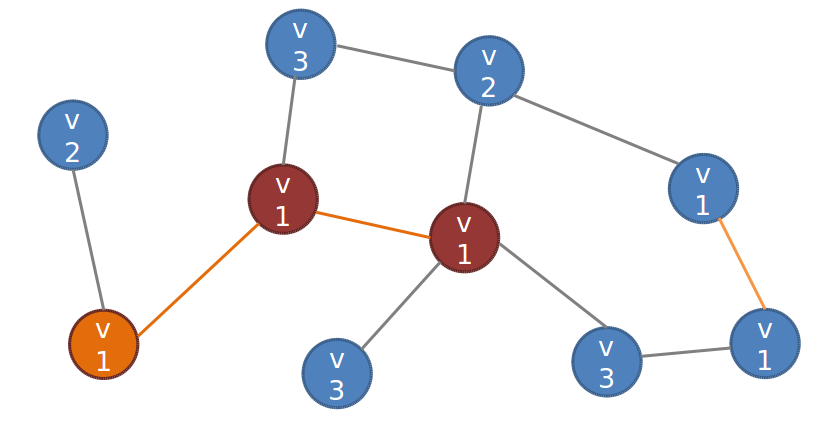
\includegraphics[width=1.0\linewidth]{Paul/python/graph.png}
     \caption{Représentation du système par un graphe}
     \label{graph}
\end{figure}

La première étape consiste à définir la répartition des logiciels dans le système. Afin de faire varier l'entropie, on utilise une distribution de Dirichlet. Celle-ci permet de s'approcher d'une distribution uniforme (proportions proches de $\frac{1}{n}$, grande entropie) ou au contraire de s'en éloigner (une proportion proche de 1 et les autres proches de 0, faible entropie). 

\begin{figure}[!ht]
\centering
     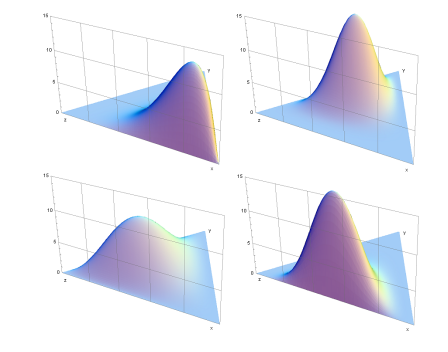
\includegraphics[width=1.0\linewidth]{Paul/python/dirichlet.png}
     \caption{Distribution de Dirichlet (source: Wikipedia)}
     \label{dirichlet}
\end{figure}

On répartit ensuite les logiciels au différents nœuds de manière aléatoire dans les proportions précédentes.
Pour chacun des logiciels du système, on prends aléatoirement l'un des nœuds sur lesquels il est présent comme le point d'entrée de l'infection. Les liens du graphe sont alors confirmés si chaque paire de nœuds correspondante est de cette version. Il ne reste alors qu'à compter le nombre de machines que l'on peut atteindre depuis la machine infectée initialement. Ce sera l'ensemble des machines infectées du système si l'attaque vise cette version.
On somme alors les cardinaux de tous ces ensembles, pondérés par la proportion de la version du logiciel correspondante dans le système.
On effectue cette simulation cent fois d'affilé pour chaque distribution, et la moyenne des résultats nous donne l'étendue moyenne de l'infection en nombre de machines infectées, pour l'entropie correspondante.

Les résultats que l'on obtient sont présentés aux figures \ref{lfixe} et \ref{nfixe}, toujours pour 100 machines.

\begin{figure}[!ht]
\centering
     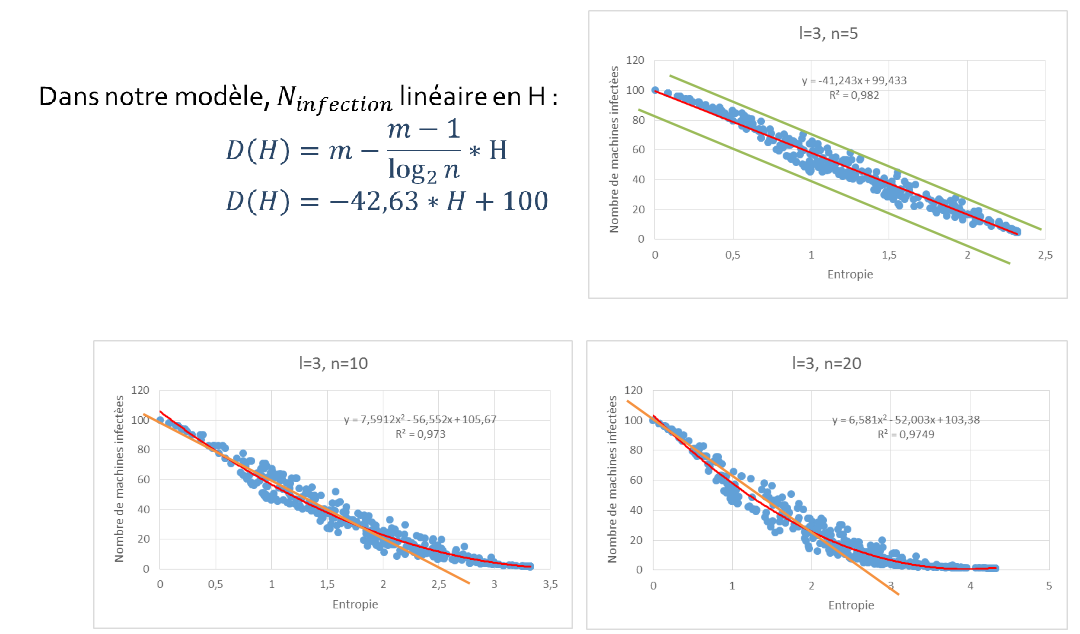
\includegraphics[width=1.0\linewidth]{Paul/python/lfixe.png}
     \caption{Simulation pour l fixé}
     \label{lfixe}
\end{figure}

Sur la figure \ref{lfixe}, on a fixé l (le degré de liaison entre les machines), mais on a fait varier n, le nombre de versions différentes dans le système. Un premier point intéressant à remarquer est qu'il y a bien une relation entre entropie et nombre de machines infectées. Pour $l=3$ et $n=5$, la relation est même linéaire, et en effectuant une régression linéaire, on obtient une droite avec des coefficients très proches de ceux obtenus avec notre modèle présenté précédemment. Celui-ci est donc bon dans ce cas précis.
Cependant, en faisant augmenter n, on constate que la décroissance du nombres de machines infectées en fonction de l'entropie se fait plutôt de manière quadratique. Mais en se restreignant à des entropies pas trop élevées (jusqu'à 2.5, ce qui sera rarement dépassé dans la réalité, cela correspondrait à quasiment installer une version différente sur chaque machine, ce qui est peu envisageable), on retrouve une approximation linéaire correcte. On peut donc en déduire que l'on peut étendre notre modèle à un nombre plus élevé de versions de logiciels, en n'augmentant pas trop l'entropie puisque de toute façon, cela a un intérêt de plus en plus réduit si elle devient trop élevée (la décroissance est alors beaucoup plus faible).

\begin{figure}[!ht]
\centering
     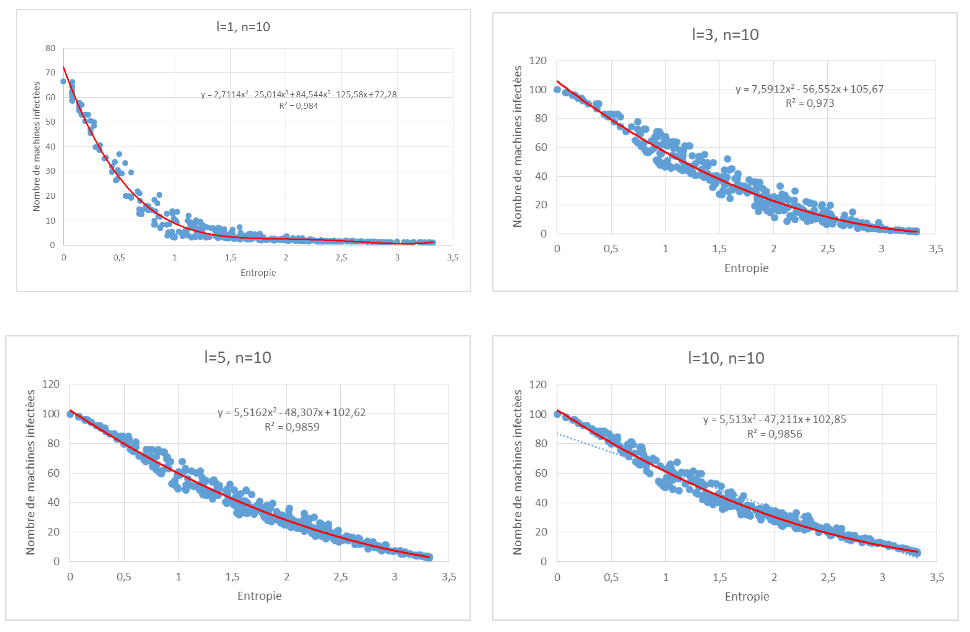
\includegraphics[width=1.0\linewidth]{Paul/python/nfixe.png}
     \caption{Simulation pour n fixé}
     \label{nfixe}
\end{figure}

Sur la figure \ref{nfixe}, on a à l'inverse fixé le nombre de versions n et fait varier le degré de liaisons l. On remarque que pour l petit, le faible nombre de liens réseau entre les machines contribue grandement à freiner la propagation du \textit{malware}. On est alors certes éloigné de notre approximation linéaire, mais on peut se contenter d'une faible entropie pour avoir une bonne défense. A partir de $l=5$ (cette valeur est relative à la taille du système en nombre m de machines), les résultats se stabilisent : il y a déjà assez de liens réseau pour que le \textit{malware} puisse se propager rapidement. C'est alors l'entropie qui redevient importante comme moyen de défense et l'on retrouve notre approximation linéaire.